\begin{task}[
  title=Maintenance of Jupyter and JupyterHub,
  id=maintenance,
  lead=SRL,
  PM=44,
  wphases={0-48},
  partners={QS,UPSUD,XFEL}
]

\begin{figure}[ht!]\centering
  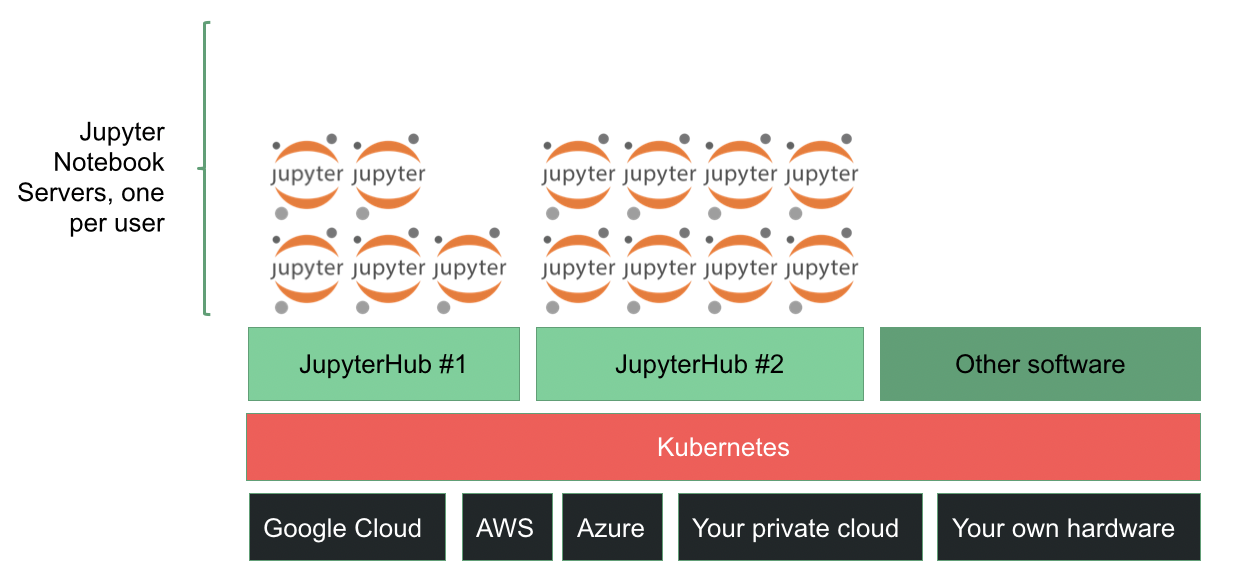
\includegraphics[width=0.6\textwidth]{images/jupyterhub-kube.png}
  \caption{
  Jupyter notebooks deployed for many users
  on shared infrastructure using JupyterHub and Kubernetes.
  }
  \label{fig:jupyterhub-kubernetes}
\end{figure}

  Developing software that people will use requires maintenance of that software,
  not just new development.
  Millions of people rely on Jupyter software,
  including all participants in \TheProject,
  and with this proposal, we fund general support of the Jupyter infrastructure.

  Maintenance of core software is often an implicit and un-paid cost,
  or one hidden in over-describing the resources required to deliver
  proposed developments.
  In \TheProject, we make it clear and explicit that we will spend a significant amount
  of time developing and maintaining the core Jupyter and JupyterHub
  e-Infrastructure to respond to the needs of \TheProject and others,
  and help keep it a healthy and active software community.

  We will contribute to supporting Jupyter e-Infrastructure software,
  ensuring that it meets the needs (\localdelivref{jupyter-contributions})
  of \TheProject,
  and aid in the release process to ensure that stable releases
  of Jupyter software can be used in mature \TheProject services
  (\localdelivref{jupyter-releases}).

  \TheProject will need improvements to core Jupyter functionality, including areas of:

  \begin{compactenum}
    \item ease of deployment
    \item security
    \item scalability of JupyterHub
    \item performance
  \end{compactenum}

  We will contribute improvements in these areas,
  meeting the needs of \TheProject and benefiting the wider Jupyter
  community.

\end{task}
